\documentclass{article}
\usepackage{amsfonts, amsmath, amssymb, amsthm} % Math notations imported
\usepackage{enumitem}
\usepackage{graphicx}
\usepackage{setspace}
\usepackage{indentfirst}
\usepackage[margin=1in]{geometry}
\graphicspath{{./images/}} % Path to images

% \begin{figure}[htb!]
%      \centering
%      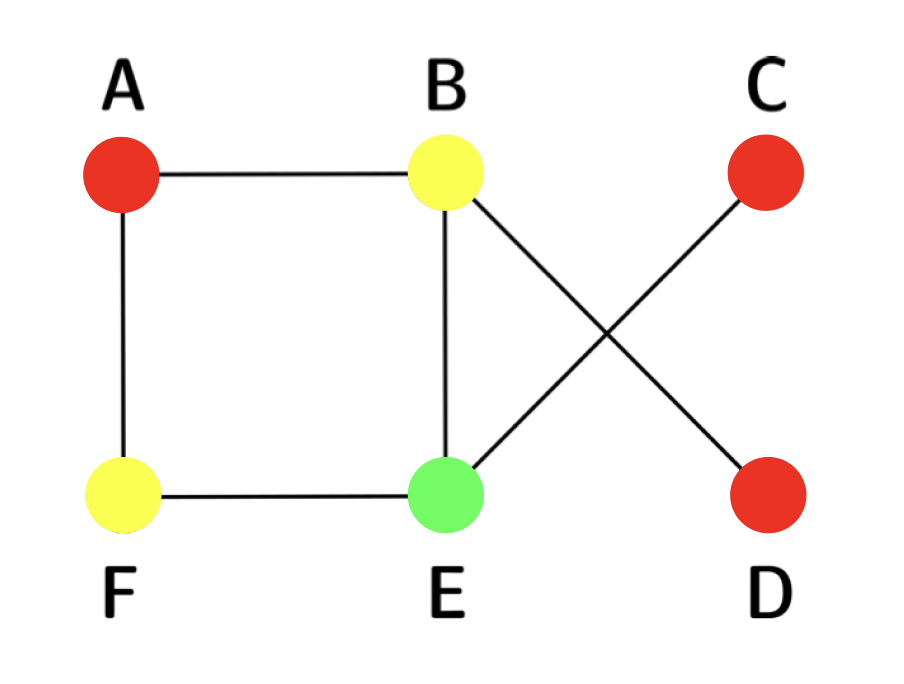
\includegraphics[scale=0.5]{coloring.png}
%      \caption{Coloring of the graph.}
% \end{figure}

% \begin{figure}[htb]
%     \qquad
%     \begin{minipage}{.4\textwidth}
%         \centering
%         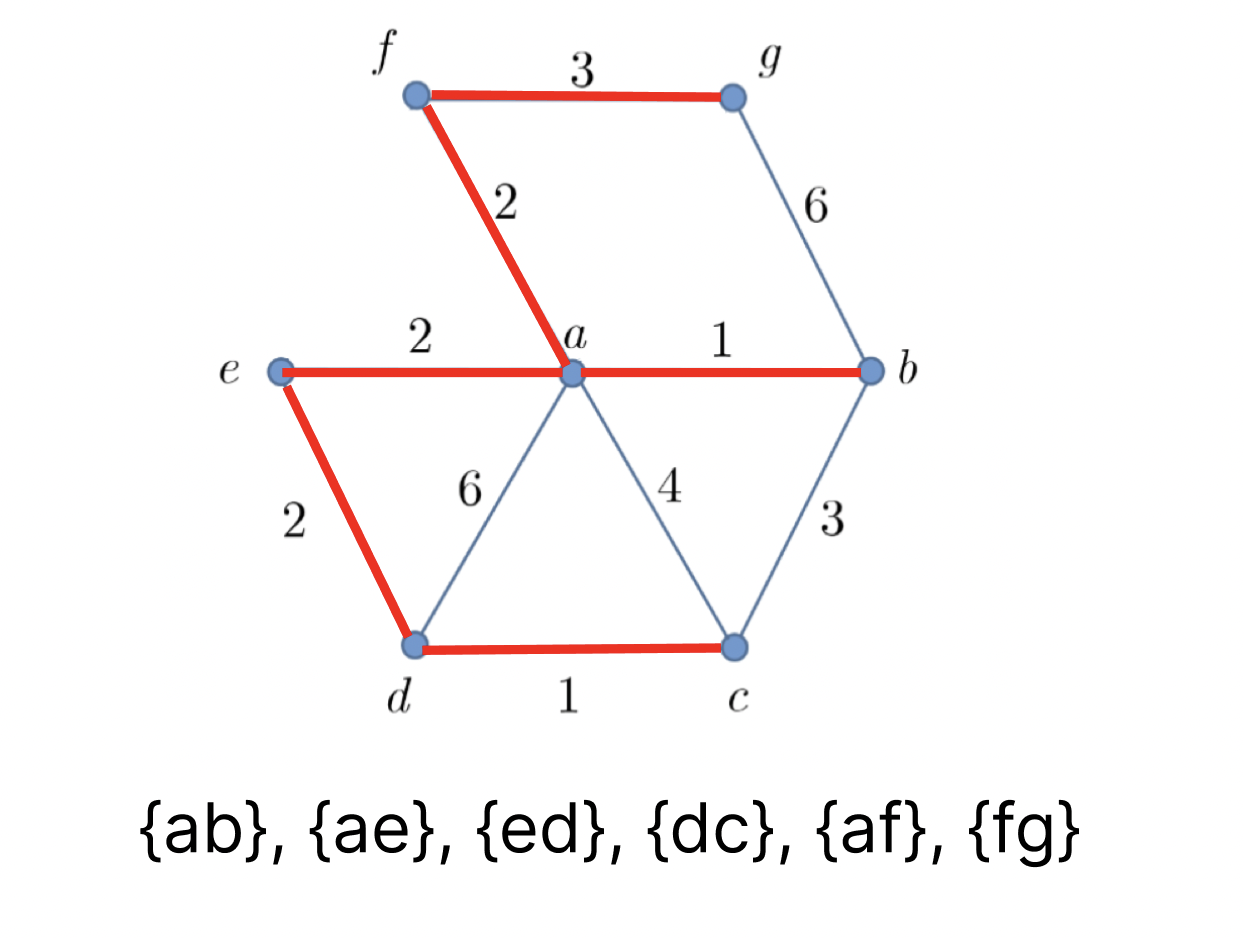
\includegraphics[scale=0.35]{prims.png}
%         \caption{}
%     \end{minipage}    
%     \qquad
%     \begin{minipage}{.4\textwidth}
%         \centering
%         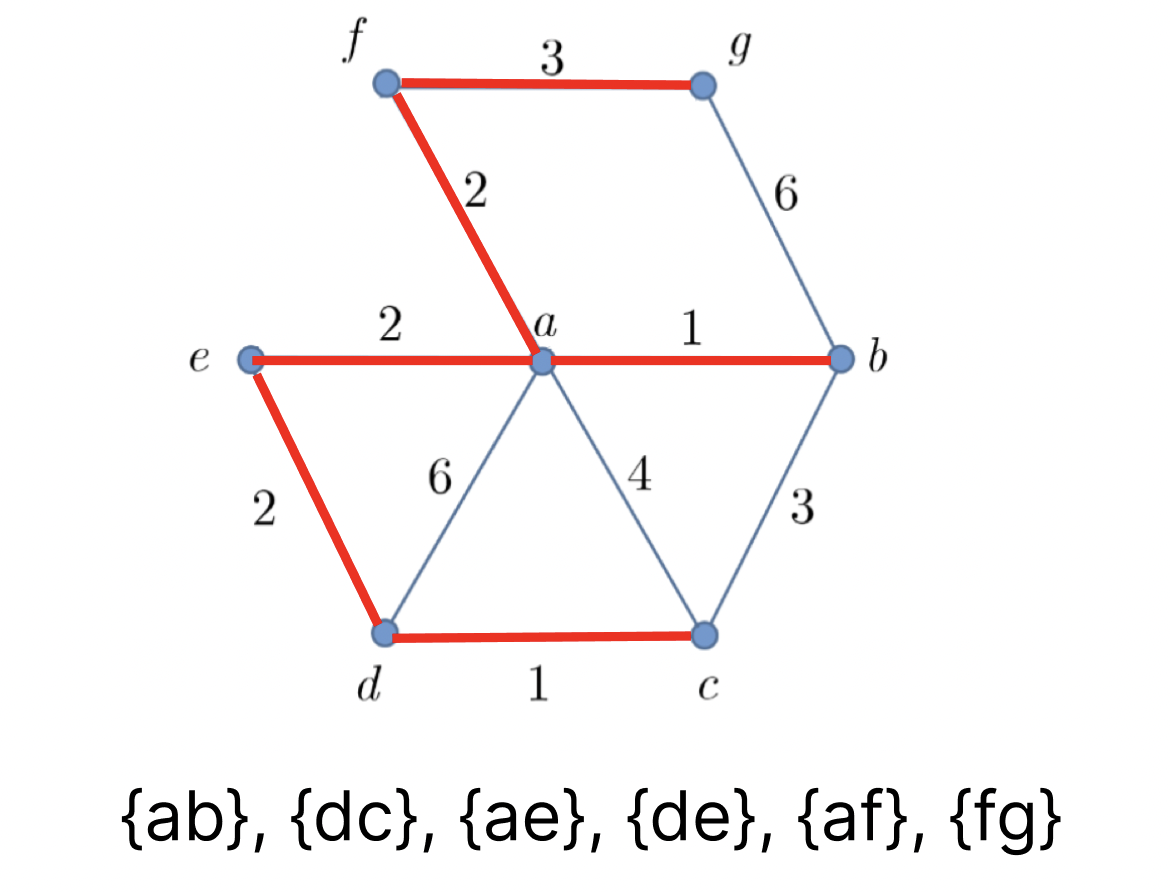
\includegraphics[scale=0.35]{kruskal.png}
%         \caption{}
%     \end{minipage}        
% \end{figure} 

\newtheorem{thm}{Theorem}
\newtheorem{proposition}[thm]{Proposition}
\newtheorem{cor}[thm]{Corollary}

% title information
\title{Math 104 Practice}
\author{Neo Lee}
\date{2023 Fall}

\setstretch{1.15}
% main content
\begin{document} 

% placing title information; comment out if using fancyhdr
\maketitle 

\section*{Chapter 14}

\begin{proposition}
    $\sum \frac{n^4}{2^n}$ converges.
\end{proposition}
\begin{proof}
    We proceed with Ratio Test.
    \begin{align*}
        \lim\left|\frac{(n+1)^4}{2^{n+1}}\cdot\frac{2^n}{n^4}\right| &= \lim\frac{(n+1)^4}{2n^4} \\
        & = \lim \frac{n^4 + O(n^3)}{2n^4} \\
        & = \frac{1}{2} < 1.
    \end{align*}
\end{proof}

\begin{proposition}
    $\sum\frac{2^n}{n!}$ converges.
\end{proposition}
\begin{proof}
    We proceed with Ratio Test.
    \begin{align*}
        \lim\left|\frac{2^{n+1}}{(n+1)!}\cdot\frac{n!}{2^n}\right| &= \lim\frac{2}{n+1} \\
        & = 0 < 1.
    \end{align*}
\end{proof}

\begin{proposition}
    $\sum\frac{n!}{n^4+3}$ diverges.
\end{proposition}
\begin{proof}
    We proceed with Ratio Test.
    \begin{align*}
        \lim\left|\frac{(n+1)!}{(n+1)^4+3}\cdot\frac{n^4+3}{n!}\right| &= \lim\frac{n(n^4+3)}{(n+1)^4+3} \\
        & = \lim\frac{n^5+3n}{n^4 + O(n^3)} \\
        & = \infty > 1.
    \end{align*}
    Hence, 
    \begin{align*}
        \lim \mathrm{inf}\left|\frac{a_{n+1}}{a_n}\right| =\lim\left|\frac{a_{n+1}}{a_n}\right| =\infty > 1.
    \end{align*}
\end{proof}

\newpage
\begin{proposition}
    $\sum\frac{cos^2n}{n^2}$ converges.
\end{proposition}
\begin{proof}
    We proceed with Comparison Test.
    \begin{align*}
        \left|\frac{cos^2n}{n^2}\right| \le \frac{1}{n^2}.
    \end{align*}
    We know $\sum\frac{1}{n^2}$ converges. Hence, $\sum\frac{cos^2n}{n^2}$ converges.
\end{proof}

\begin{proposition}
    $\sum_{n=2}^{\infty}\frac{1}{log n}$ diverges.
\end{proposition}
\begin{proof}
    We proceed with Comparison Test.
    \begin{align*}
        \frac{1}{log n} \ge \frac{1}{n}.
    \end{align*}
    We know $\sum_{n=2}^\infty\frac{1}{n}$ diverges to $+\infty$. Hence, 
    $\sum_{n=2}^\infty\frac{1}{log n}$ diverges to $+\infty$.
\end{proof}

\begin{proposition}
    Suppose $\sum a_n=A, \sum b_n=B$  where $A, B \in \mathbb{R}$. Then, $\sum (a_n+b_n)=A+B$.
\end{proposition}
\begin{proof}
    Define $(a'_n)$ as the partial sums of $(a_n)$, $(b'_n)$ as the partial sums of $(b_n)$, and 
    $(c'_n)$ as the partial sums of $(a_n+b_n)$. 
    Then
    \begin{align*}
        \sum(a_n+b_n) & = \lim c'_n \\
        & = \lim (a'_n + b'_n) \\
        & = \lim a'_n + \lim b'_n \\
        & = A + B.
    \end{align*}
\end{proof}

\begin{proposition}
    Suppose $\sum a_n=A$  for $A \in \mathbb{R}$. Then, $\sum ka_n=kA$ for 
    $k \in \mathbb{R}$.
\end{proposition}
\begin{proof}
    Define $(a'_n)$ as the partial sums of $(a_n)$ and 
    $(c'_n)$ as the partial sums of $(ka_n)$. 
    Then
    \begin{align*}
        \sum(ka_n) & = \lim c'_n \\
        & = \lim (ka'_n) \\
        & = k\lim a'_n \\
        & = kA.
    \end{align*}
\end{proof}

\begin{proposition}
    Suppose $\sum a_n=A, \sum b_n=B$  where $A, B \in \mathbb{R}$. Then, $\sum (a_n\cdot b_n)=AB$
    is not true in general.
\end{proposition}
\begin{proof}
    Define $(a_n) = (1, 0, 0, 0, \dots), (b_n) = (1/2)^n$. Then $A=1, B=2$ and $AB = 2$. But notice 
    $a_n\cdot b_n = 0$ for all $n\neq 0$ and $\sum(a_n\cdot b_n) = a_0\cdot b_0 = 1\neq AB = 2$.
\end{proof}

\newpage
\begin{proposition}
    If $\sum|a_n|$ converges and $(b_n)$ is a bounded sequence, then $\sum a_nb_n$ converges.
    Note: Corollary 14.7 that absolutely convergent series are convergent is a special case when 
    $(b_n)$ is taken to be 1 for all $n$.
\end{proposition}
\begin{proof}
    Since $(b_n)$ is bounded, we know there exists an supremum for $(|b_n|)$, denote 
    $M = max\{\sup(|b_n|),1\}$. Then, we know there exists $N\in\mathbb{N}$ such that for $n\ge m>N$, 
    $\sum_{k=m}^n|a_k|<\frac{\epsilon}{M}$ for all $\epsilon>0$. Now, take such $N$ and
    \begin{align*}
        \sum_{k=m}^n|a_k| & < \frac{\epsilon}{M} \\
        M\sum_{k=m}^{n}|a_k| & < \epsilon \\
        \left|\sum_{k=m}^{n}a_kb_k\right| \le \sum_{k=m}^{n}|a_k||b_k| \le \sum_{k=m}^{n}|a_k|M & < \epsilon.
    \end{align*}
    Hence, $\sum a_nb_n$ satifies the Cauchy criterion and thus converges.
\end{proof}

\begin{proposition}
    If $\sum a_n$ is a convergent series of nonnegative numbers and $p>1$, then $\sum a^p_n$ 
    converges.
\end{proposition}
\begin{proof}
    We know there exists $N$ such that for $n\ge m>N$, 
    $\left|\sum_{k=m}^{n}a_k\right|<\sqrt[p]{\epsilon}$ for all $\epsilon>0$.
    Take some $\epsilon>0$ and such $N$, then
    \begin{align*}
        \left|\sum_{k=m}^{n}a_k\right| & < \sqrt[p]{\epsilon} \\
        \left|\sum_{k=m}^{n}a_k\right|^p & < \epsilon \\
        \left|\sum_{k=m}^na_k^p\right| \le \left|\left(\sum_{k=m}^na_k\right)^p\right| & < \epsilon.
    \end{align*}
    Hence, $\sum a_n^p$ satifies Cauchy criterion and thus converges.
\end{proof}

\newpage
\begin{proposition}
    If $\sum a_n$ and $\sum b_n$ are convergent series of nonnegative numbers, then 
    $\sum\sqrt{a_nb_n}$ converges. Hint: show $\sqrt{a_nb_n}\le a_n+b_n$ for all $n$.
\end{proposition}
\begin{proof}
    Notice for all $n$
    \begin{align*}
        a_n^2 + b_n^2 + 2a_nb_n & \ge a_nb_n\\
        \left(a_n+b_n\right)^2 & \ge a_nb_n \\
        a_n + b_n & \ge \sqrt{a_nb_n}.
    \end{align*}

    Also, we know there exists $N_1$ such that for $n\ge m>N_1$, 
    $\left|\sum_{k=m}^na_k\right|<\epsilon/2$ and $N_2$ such that for $n\ge m>N_2$, 
    $\left|\sum_{k=m}^nb_k\right|<\epsilon/2$. Now we take $N = \max\{N_1,N_2\}$ for some 
    $\epsilon>0$. Then, for all $n\ge m>N$
    \begin{align*}
        \left|\sum_{k=m}^n\sqrt{a_nb_n}\right| & \le \left|\sum_{k=m}^{n}a_k+b_k\right| \\
        & \le \left|\sum_{k=m}^{n}a_k+\sum_{k=m}^{n}b_k\right| \\
        & \le \left|\sum_{k=m}^{n}a_k\right| + \left|\sum_{k=m}^{n}b_k\right| \\
        & < \epsilon.
    \end{align*}
    Hence, $\sum\sqrt{a_nb_n}$ satisfied Cauchy criterion and thus converges.
\end{proof}

\begin{proposition}
    The convergence of a series does not depend on any finite number of terms, though the 
    value of the limit does. More precisely, consider series $\sum a_n$ and $\sum b_n$ and suppose 
    that the set $\{n\in\mathbb{N}:a_n\neq b_n\}$ is finite. Then the series both converge or else 
    the both diverge.
\end{proposition}
\begin{proof}
    Without loss of generality, we will focus on $\sum a_n$ and conclude the convergence of 
    $\sum b_n$ based on $\sum a_n$. Also, denote $M=\max\{n\in\mathbb{N}:a_n\neq b_n\}$.

    \underline{Case 1: $\sum a_n$ converges.} We know $\sum a_n$ satisfies Cauchy criterion, 
    thus we know there exists $N_1$ such that for all $n\ge m>N_1$, 
    $\left|\sum_{k=m}^{n}a_k\right|<\epsilon$ for some $\epsilon>0$. 
    
    Then, let 
    $N_2=\max\{N_1, M\}$. Since we have set $N_2$ to be at least $M$, any terms after $N_2$ for 
    $b_n$ is the same as $a_n$. Thus, any statement that holds true for $a_n$ is also true for $b_n$
    after $N_2$ and we can conclude for all $n\ge m>N_2$ $\left|\sum_{k=m}^{n}b_k\right|<\epsilon$ 
    for some $\epsilon>0$.

    Therefore, $\sum b_n$ satifies Cauchy criterion too and thus converges.

    \underline{Case 2: $\sum a_n$ diverges.} Assume for the sake of contradiction that $\sum b_n$ 
    converges. Then there exists $N_2$ for all $\epsilon>0$ such that for $n\ge m>N_2$, 
    $\left|\sum b_n\right|<\epsilon$. Thus, we can take $N_1=\max\{N_2,M\}$, which will make sure 
    that for $n\ge m>N_1$, $\left|\sum_{k=m}^n a_n\right|<\epsilon$ for each $\epsilon$. 
    But that contradicts that fact that $\sum a_n$ diverges. Hence, $\sum b_n$ must diverge.
\end{proof}

\begin{proposition}
    Let $(a_n)$ be a sequence of nonzero real numbers such that the sequence 
    $\left(\frac{a_{n+1}}{a_n}\right)$ of ratios is a constance sequence, then $\sum a_n$ is a 
    geometric series.
\end{proposition}
\begin{proof}
    Let $r = \frac{a_{n+1}}{a_n}$ for all $n$. Then we can define $(a_n)$ recursively such that 
    $a_{n+1} = a_n\cdot r$. Hence, $a_n=a_0\cdot r^n$. Indeed, 
    $$\sum a_n = \sum_{k=0}^{n}a_0\cdot r^k,$$ which is a geometric series.
\end{proof}

\begin{proposition}
    Let $(a_n)_{n\in\mathbb{N}}$ be a sequence such that $\lim\inf |a_n|=0$, then there is a 
    subsequence such that $\sum_{k=1}^{\infty}a_{n_k}$ converges.
\end{proposition}
\begin{proof}
    Since $\lim\inf |a_n|=0$, we know there exists a subsequence of $(|a_n|)$ that converges to 0. 
    Hence, for each $\epsilon$, the set $\{n:\mathbb{N}:|a_n|<\epsilon\}$ is infinite. Then 
    we can construct a subsequence such that $\sum_{k=1}^{\infty}a_{n_k}$ converges.

    For each $k+1$, choose $n_{k+1}>n_k$ such that $|a_{n_{k+1}}|<\frac{1}{2^{k+1}}=b_{k+1}$. Then, 
    for each $k$, $|a_{n_k}|\le b_k$. Apparently, $\sum b_k$ is a convergent geometric series, thus 
    by comparison test, $\sum_{k=1}^\infty a_{n_k}$ converges.
\end{proof}

\begin{proposition}
    $\sum_{n=1}^{\infty}\frac{1}{n(n+1)}=1$. Hint: $\sum_{k=1}^{n}\frac{1}{k(k+1)}=
    \sum_{k=1}^{n}\left(\frac{1}{k}-\frac{1}{k+1}\right)$.
\end{proposition}
\begin{proof}
    Notice 
    \begin{align*}
        \sum_{k=1}^{n}\frac{1}{k(k+1)} & = \sum_{k=1}^{n}\left(\frac{1}{k}-\frac{1}{k+1}\right) \\
        & = \left(1-\frac{1}{2}\right) + \left(\frac{1}{2}-\frac{1}{3}\right) + \dots +
        \left(\frac{1}{n}-\frac{1}{n+1}\right) \\
        & = 1 - \frac{1}{n+1}.
    \end{align*}
    Hence, 
    \begin{align*}
        \sum_{n=1}^{\infty}\frac{1}{n(n+1)} & = \lim_{n\to\infty}\sum_{k=1}^{n}\frac{1}{k(k+1)} \\
        & = \lim_{n\to\infty}\left(1 - \frac{1}{n+1}\right) \\
        & = 1.
    \end{align*}
\end{proof}

\begin{proposition}
    $\sum_{n=1}^{\infty}\frac{n-1}{2^{n+1}}=\frac{1}{2}$. 
    Hint: $\frac{k-1}{2^{k+1}}=\frac{k}{2^k}-\frac{k+1}{2^{k+1}}$.
\end{proposition}
\begin{proof}
    Notice 
    \begin{align*}
        \sum_{k=1}^{n}\frac{k-1}{w^{k+1}} & = 
        \sum_{k=1}^{n}\left(\frac{k}{2^k}-\frac{k+1}{2^{k+1}}\right) \\
        & = \left(\frac{1}{2}-\frac{2}{2^2}\right) + \left(\frac{2}{2^2}-\frac{3}{2^3}\right) 
        + \cdots + \left(\frac{n}{2^n}-\frac{n+1}{2^{n+1}}\right) \\
        & = \frac{1}{2} - \frac{n+1}{2^{n+1}}.
    \end{align*}

    Hence, 
    \begin{align*}
        \sum_{n=1}^{\infty}\frac{n-1}{2^{n+1}} & = \lim_{n\to\infty}\sum_{k=1}^{n}\frac{k-1}{2^{k+1}} \\
        & = \lim_{n\to\infty}\left(\frac{1}{2} - \frac{n+1}{2^{n+1}}\right) \\
        & = \frac{1}{2} - \lim_{k\to\infty}\frac{k}{2^k} \\
        & = \frac{1}{2} - \lim_{k\to\infty}\left(\frac{\sqrt[k]{k}}{2}\right)^k \\
        & = \frac{1}{2}.
    \end{align*}
\end{proof}

\begin{proposition}
    SHow that $\sum_{n=1}^{\infty}\frac{1}{n}$ diverges by comparing with the series 
    $\sum_{n=2}^{\infty}a_n$ where $(a_n)$ is the sequence 
    $$(\frac{1}{2},\frac{1}{4},\frac{1}{4},\frac{1}{8},\frac{1}{8},\frac{1}{8},\frac{1}{8}
    ,\frac{1}{16},\frac{1}{16},\frac{1}{16},\frac{1}{16},\frac{1}{16},\frac{1}{16},\frac{1}{16}
    ,\frac{1}{16},\frac{1}{32},\frac{1}{32}, \cdots).$$
\end{proposition}
\begin{proof}
    We will show that $\sum_{n=2}^{\infty}\frac{1}{n}$ diverges and thus 
    $\sum_{n=1}^{\infty}\frac{1}{n}$, which differs only by the first term.

    Notice for all $2^k< n\le2^{k+1}$, $a_n = \frac{1}{2^{k+1}}\le\frac{1}{n}$. This is true for 
    all $k\in\mathbb{N}$. Hence, $\frac{1}{n}\le a_n$ for all $n$. Now observe within each interval 
    $(2^k,2^{k+1}]$, there are $2^k$ terms. Therefore, $\sum_{n=2^k}^{2^{k+1}}a_n=\frac{1}{2}$ and 
    $\sum_{n=2}^{\infty}a_n = \lim_{k\to\infty}k\left(\frac{1}{2}\right)=\infty$. 

    Hence, by Comparison Test, $\sum_{n=1}^{\infty}\frac{1}{n}$ also diverges.
\end{proof}

\end{document}
